\chapter{Introducción Específica} % Main chapter title

\label{Chapter2}

%----------------------------------------------------------------------------------------
La idea de este capítulo es presentar una visión general del equipo desarrollado y mostrar algunos aspectos de la planificación del proyecto.


\section{Esquema general del sistema}

El producto básicamente debe permitir controlar una carga eléctrica a través de comandos que se le envían desde un teléfono móvil. Un esquema básico del sistema puede verse en la Figura \ref{fig:esquema_sistema}. Dentro del contexto de este trabajo final, se desarrolló un prototipo funcional del equipo. Por lo tanto, es un producto que cumple todas la funciones que va a tener el equipo final, pero que no busca cumplir con características mecánicas y estéticas que si van a estar presentes en el producto comercial. Una descripción detallada del hardware desarrollado se encuentra en la Sección \ref{section:hardware}.

\begin{figure}[h]
	\centering
	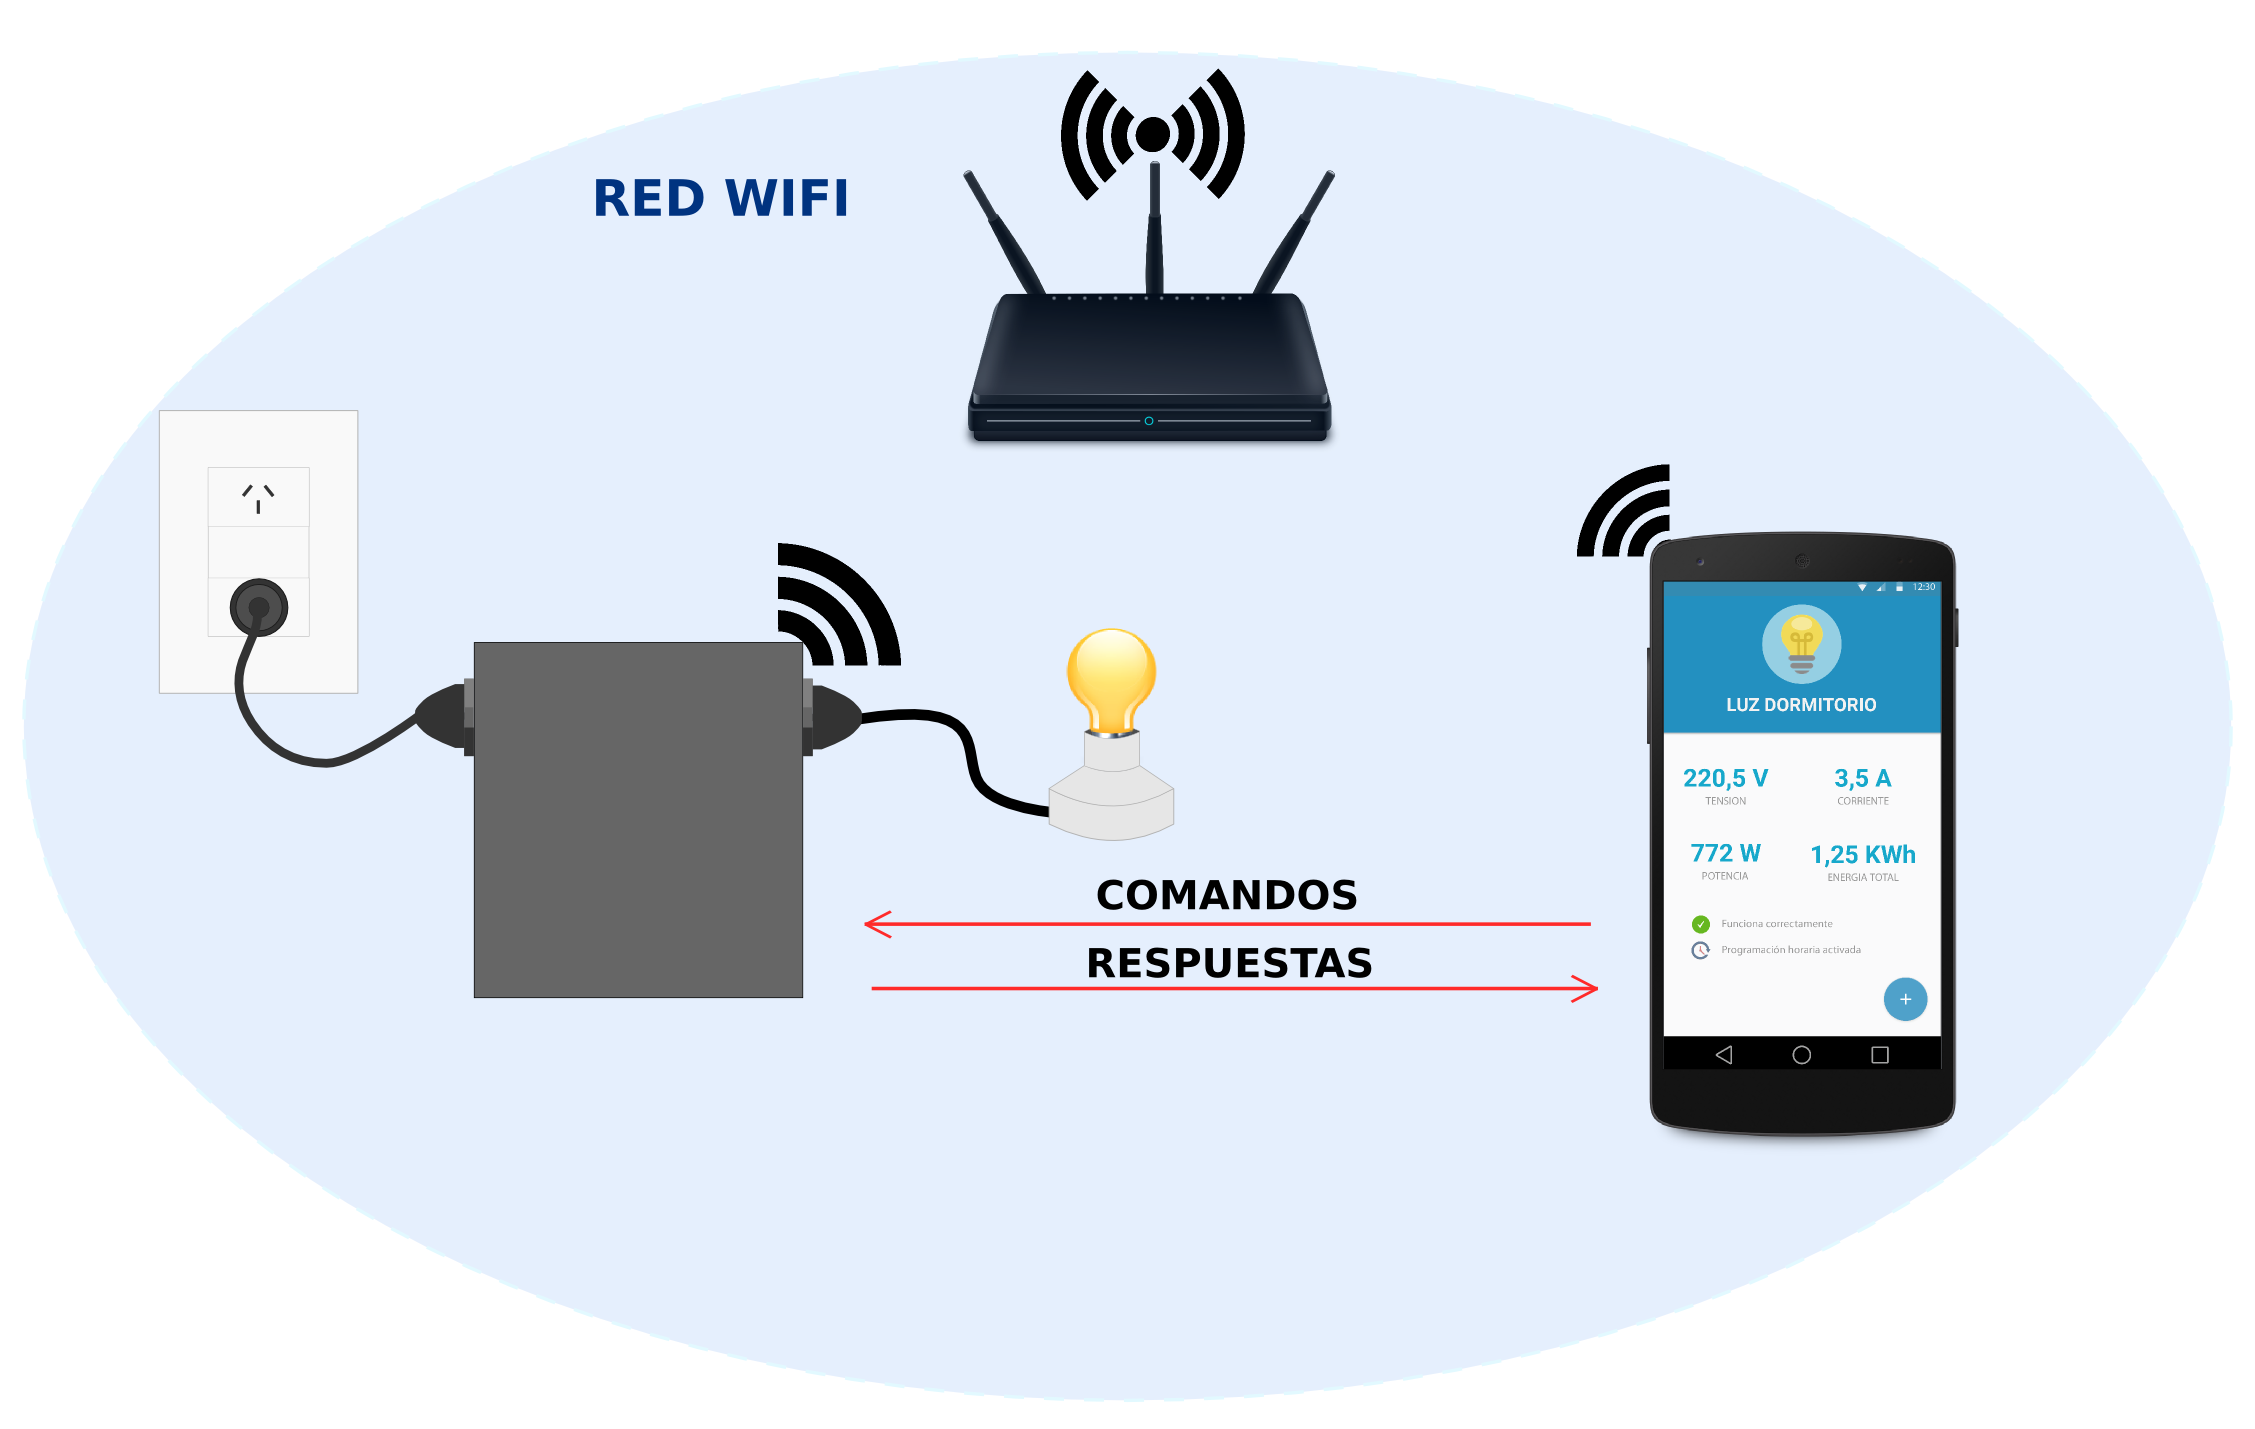
\includegraphics[width=12cm]{./Figures/2_1_esquema_sistema.png}
	\caption{Esquema general del sistema propuesto en este proyecto, compuesto por un Smart Plug y la aplicación móvil.}
	\label{fig:esquema_sistema}
\end{figure}

Cuando se adquiere un Smart Plug, lo primero que debe hacerse es incorporarlo a la red WiFi del hogar. Se eligió que la comunicación fuera a través de esta red, ya que con el paso de los años cada vez es más común que en las casas esté disponible este servicio, debido a que muchos otros dispositivos electrónicos necesitan de una conexión a Internet.

Para agregar el Smart Plug a la red, se puede proceder de dos formas: WPS o configurando la red en el Smart Plug. En el primer caso, el proceso es sumamente sencillo: simplemente se debe presionar el pulsador que se encuentra en la placa del Smart Plug (el led verde comenzará a destellar) y luego presionar el pulsador de WPS que se encuentra en el router WiFi. Una vez hecho esto, el Smart Plug se incorpora a la red. 

Sin embargo, muchos routers hogareños no cuentan con la funcionalidad de WPS, por lo que existe otra forma de configurar la red WiFi. Esta consiste en establecer al Smart Plug como un punto de acceso temporario. Para esto se debe mantener presionado el pulsador en la placa del Smart Plug durante 5 segundos. Cuando el led verde comienza a destellar, indica que el punto de acceso fue creado. Luego de esto se debe conectar un dispositivo móvil a la red WiFi creada por el Smart Plug. Una vez conectado, mediante un \textit{browser} se debe entrar a la página de configuración de la red WiFi (\textit{http://config}) y cargar los parámetros de la red a la que se desea conectar el Smart Plug: SSID de la red, tipo de seguridad y clave.

Cuando el Smart Plug se encuentra conectado a la red WiFi ya puede comenzar a ser comandado mediante la aplicación móvil. El único requerimiento para que el sistema funcione es que tanto los Smart Plugs como el teléfono en el que está la aplicación se encuentren en la misma red WiFi. En el alcance de este trabajo no estaba contemplado el desarrollo de la infraestructura para poder comandar los Plugs desde fuera del hogar.

La aplicación lista todos los Plugs que encuentra en la red WiFi y permite: encender/apagar la carga, conocer algunos parámetros eléctricos (tensión corriente, potencia y energía), configurar horarios de encendido y apagado, visualizar mediciones históricas de potencia y energía. La cantidad de Smart Plugs que puede gestionar la aplicación no está limitada, por lo que se pueden controlar numerosos dispositivos eléctricos dentro de una casa.

Además de poder enviar comandos a los Smart Plugs cuando el usuario lo requiere, la aplicación inicia un servicio en Android que se encarga de realizar consultas periódicamente a todos los Smart Plugs que tiene registrados, aun cuando la aplicación se encuentre cerrada. Mediante estas consultas, la aplicación va a poder conocer: si la carga está encendida o no, las últimas mediciones, los cambios en las configuraciones del equipo, etc. De esta forma se logra que una aplicación móvil puedan comandar y configurar un Smart Plug y todas las demás que tengan registrado a ese mismo Plug se mantengan actualizadas con estos cambios. Una explicación más detallada del funcionamiento y del diseño de la aplicación móvil se encuentra en la Sección \ref{section:app}.

Finalmente, la comunicación entre los Smart Plugs y la aplicación móvil se basa en conexiones TCP iniciadas por la aplicación. Sobre TCP se desarrolló un protocolo propio que permite enviar comandos a los Plugs tanto para que realicen acciones como para leer/escribir valores de ciertos registros también definidos por el protocolo diseñado. Este protocolo es explicado en mayor profundidad en la Subsección \ref{subsection:protocolo}.



\section{Requerimientos}
\label{sec:requerimientos}

A continuación se enumeran los requerimientos de hardware, firmware y de la aplicación móvil. Inicialmente se habían planteado un número mucho más reducido de requerimientos. Así también eran requerimientos que debían ser divididos en otros más acotados para facilitar su validación. Antes de comenzar con el desarrollo del producto, se establecieron claramente estos requerimientos, para lo cual fueron importantes los aportes realizados desde las áreas de marketing (en cuanto al aspecto estético y funcionalidades deseadas) y de atención al cliente (en base a comentarios de los clientes referidos a un producto de estas características).

\begin{itemize}
\item Requerimientos de Hardware

\begin{itemize}
\item Req \#1.1: El Smart Plug debe poder operar con cargas de 220VAC y hasta 5A.
\item Req \#1.2: La fuente de alimentación debe generar 5V y 3,3V
\item Req \#1.3: La fuente de alimentación debe entregar 350mA.
\item Req \#1.4: El encendido y apagado de la carga se realizará con un relay mecánico de 5V. Se deben usar los contactos común y normal cerrado.
\item Req \#1.5: La interfaz de programación debe ser accesible mediante un header de pines.
\item Req \#1.6: Utilizar un front-end analógico monolítico para realizar el análisis de los parámetros eléctricos.
\item Req \#1.7: Conectarse a la red hogareña mediante un módulo WiFi.
\item Req \#1.8: Debe poseer un pulsador de tipo tact switch. El presionarlo pone un nivel lógico alto.
\item Req \#1.9: Debe poseer un led bicolor verde y rojo. Se encienden independientemente con un nivel lógico alto.
\item Req \#1.10: Deberá tener una memoria EEPROM SPI de la línea 25LC de Microchip.
\end{itemize}

\item Requerimientos de Firmware

\begin{itemize}
\item Req \#2.1: Cuando se inicia el modo WPS, el led verde debe destellar a una frecuencia aproximada de 1Hz.
\item Req \#2.2: Cuando se inicia el modo Soft-AP, el led verde debe destellar a una frecuencia aproximada de 2Hz.
\item Req \#2.3: Cuando se une a una red WiFi, si logra sincronizar la hora con el servidor NTP, el led verde se debe encender.
\item Req \#2.4: Cuando se une a una red WiFi, si no logra sincronizar la hora con el servidor NTP, el led verde y el rojo deben destellar.
\item Req \#2.5: Si no se puede unir a una red WiFi, el led rojo debe destellar a una frecuencia aproximada de 1Hz.
\item Req \#2.6: Al presionar el botón de la placa se debe iniciar el proceso de WPS.
\item Req \#2.7: Al mantener presionado por 5 segundos el botón de la placa se debe iniciar el Soft-AP.
\item Req \#2.8: Si se desconecta el Smart Plug, cuando se lo vuelve a conectar se debe intentar unir a la última red WiFi a la que estuvo unido.
\item Req \#2.9: Al conectarse a una red WiFi, se debe conectar a un servidor NTP y obtener la fecha y la hora.
\item Req \#2.10: La fecha y la hora deben ser llevadas por un RTC en el microcontrolador.
\item Req \#2.11: Debe existir un módulo encargado de registrar la actividad en el equipo. Su salida va a ser una UART configurada a 115200 baud - 8N1.
\item Req \#2.12: Se deben obtener las siguientes mediciones de la línea: tensión eficaz, corriente eficaz, potencia activa, frecuencia, factor de potencia y energía. 
\item Req \#2.13: El intervalo entre una muestra y la siguiente de cada medición no debe superar los 10 segundos.
\item Req \#2.14: Cada hora el Smart Plug debe obtener la potencia activa promedio de esa hora y la energía de esa hora.
\item Req \#2.15: Cada hora se deben guardar de forma no volátil las mediciones de potencia activa y energía correspondientes a esa hora.
\item Req \#2.16: Se deben guardar de forma no volátil las mediciones de potencia activa y energía correspondiente a las 24 horas de los últimos 7 días.
\item Req \#2.17: Cada dispositivo debe tener un ID único de 6 dígitos hexadecimales cargado durante la prueba de fábrica.
\item Req \#2.18: Cada dispositivo debe guardar de forma no volátil un nombre de hasta 32 caracteres.
\item Req \#2.19: Debe guardar de forma no volátil los parámetros de calibración del front-end analógico.
\item Req \#2.20: Debe permitir configurar una hora de encendido y apagado de la carga para cada día de la semana.
\item Req \#2.21: Cuando llega la hora de encendido configurada para el día correspondiente, la carga se debe encender.
\item Req \#2.22: Cuando llega la hora de apagado configurada para el día correspondiente, la carga se debe apagar.
\item Req \#2.23: Cuando el dispositivo se inicia debe chequear que la EEPROM esté inicializada. Debe haber un valor “bandera” en la EEPROM que indique si está inicializada.
\item Req \#2.24: Si la memoria EEPROM no está inicializada se deben cargar los siguientes valores: nombre - Smart Plug; horarios de encendido y apagado - 0:0.
\item Req \#2.25: El Smart Plug debe generar un mensaje UDP periódicamente para darse a conocer en la red WiFi. Lo debe enviar a la dirección broadcast.
\item Req \#2.26: En el mensaje periódico se debe indicar número de ID.
\item Req \#2.27: La comunicación con la App móvil va a ser a través de mensajes sobre TCP. Se debe respetar el formato de la trama definido en [1].
\end{itemize}

\item Requerimientos App móvil

\begin{itemize}
\item Req \#3.1: Debe identificar los Smart Plugs presenten en la red.
\item Req \#3.2: Debe permitir encender y apagar cada Smart Plug.
\item Req \#3.3: Debe mostrar el estado actual de la carga: encendida o apagada.
\item Req \#3.4: Debe mostrar el estado de la comunicación con cada Smart Plug: comunicación OK o con errores.
\item Req \#3.5: Debe mostrar la hora y la fecha de la última comunicación exitosa con cada Smart Plug. 
\item Req \#3.6: Debe permitir configurar el nombre de cada Smart Plug encontrado.
\item Req \#3.7: Debe permitir configurar el horario de encendido y apagado de la carga para cada día de la semana.
\item Req \#3.8: Debe permitir deshabilitar la programación horaria para cada día de la semana.
\item Req \#3.9: Debe permitir asignar un ícono a cada Smart Plug.
\item Req \#3.10: Debe permitir visualizar las mediciones de: tensión eficaz, corriente eficaz, potencia activa y energía acumulada. Para cada Smart Plug.
\item Req \#3.11: Debe permitir visualizar las mediciones históricas de potencia activa y energía de los últimos 20 días mediantes gráficos del tipo “Magnitud vs. hora del día”.
\item Req \#3.12: Debe permitir borrar las mediciones históricas y la energía acumulada en los Smart Plugs.
\item Req \#3.13: Debe permitir volver a valores de fábrica a los Smart Plugs.
\item Req \#3.14: Debe actualizar de forma periódica (cada 10 minutos) la información de cada Smart Plug. La información incluye: nombre del dispositivo, estado de la carga, tensión eficaz, corriente eficaz, potencia activa y energía acumulada.
\item Req \#3.15: Debe actualizar de forma periódica (cada 1 hora) las mediciones por hora de la potencia activa y energía de cada Smart Plug.
\item Req \#3.16: La actualización periódica debe continuar aún cuando la aplicación esté cerrada.
\end{itemize}

\end{itemize}



\section{Planificación}

En la Figura \ref{fig:diagrama_gantt} puede observarse el diagrama de Gantt con la tareas realizadas en el contexto de este proyecto.

\begin{figure}[!h]
	\centering
	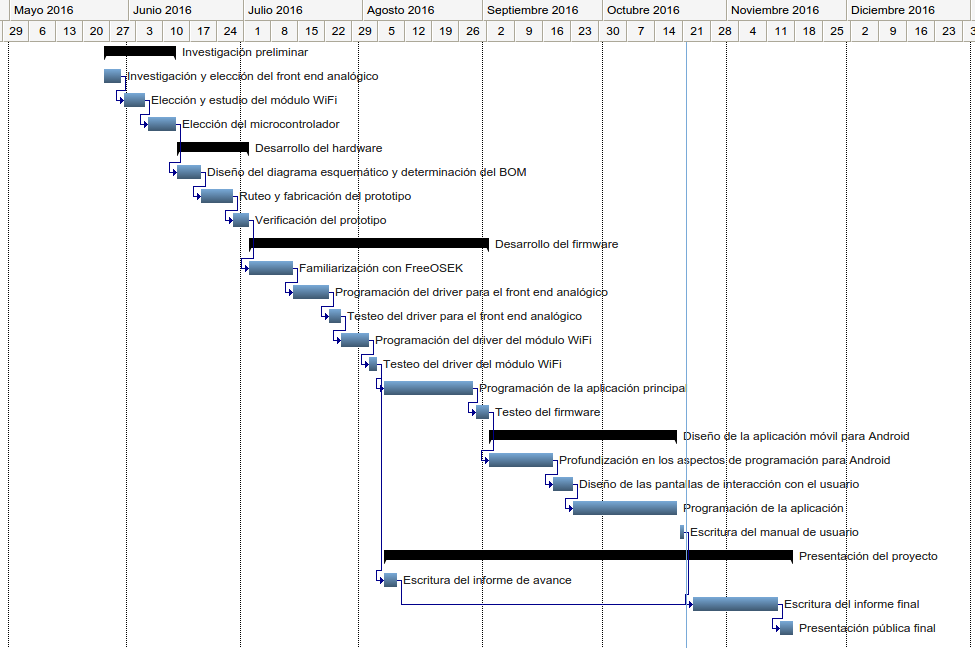
\includegraphics[width=18cm, angle=90]{./Figures/2_3_diagrama-Gantt.png}
	\caption{Diagrama de Gantt de la planificación del proyecto.}
	\label{fig:diagrama_gantt}
\end{figure}


Para mayor información acerca de la planificación se puede recurrir al documento \textit{Planificación del Trabajo Final de Carrera - Mondani Mariano} en \citep{repo_planificacion}, en donde se puede encontrar la planificación detallada, incluyendo las tareas y los riesgos que se contemplaron al iniciar el proyecto.
